\section{Premiers graphes avec tkz-graph.sty}

 \tkzname{TikZ} est un outil que je trouve très agréable à utiliser pour la création de graphes. J'ai trouvé si simple son utilisation que je me suis demandé si cela avait un sens de créer un package pour  la création de graphes. Pas de théorie des graphes dans ce package, seulement des outils pour leur construction.  Trois arguments peuvent intervenir pour soutenir mon effort :

\begin{enumerate}

\item Certains utilisateurs n'ont pas envie d'apprendre quoi que ce soit sur  \TIKZ\; cela est respectable et une simplification du code par l'intermédiaire d'un package peut avoir une certaine utilité. La syntaxe n'est plus tout à fait celle de  \TIKZ\ mais celle de \LATEX.
\item Il est possible finalement de jouer avec les styles et d'optimiser certains situations, ainsi la création d'un graphe sans la moindre coordonnée est possible. On peut obtenir des variantes du graphe, simplement en jouant avec les styles.
\item  La création de ce que l'on peut appeler les graphes classiques de la théorie des graphes.
\item  Et pour terminer, cela peut être une approche en douceur de l'utilisation de \TIKZ\, par l'intermédiaire des options.

\end{enumerate}

Que peut apporter \tkzname{tkz-graph.sty} ? Il  facilite la gestion des styles des sommets  et des arêtes, et également le positionnement de ceux-ci.

\subsection{Exemple simple avec \tkzname{tkz-graph}}
Avant d'expliquer le fonctionnement des différentes macros, il est possible de tester si le package est bien installé avec l'exemple simple suivant. Le code complet est donné. Le préambule peut évidemment être modifié.


\medskip
\begin{minipage}{.45\textwidth}
\begin{tkzltxexample}[]
% Author   : Alain Matthes
% Encoding : UTF8
% Engine   : LuaLaTeX
\documentclass[border=3mm]{standalone}
\usepackage{tkz-graph}
\begin{document}
  
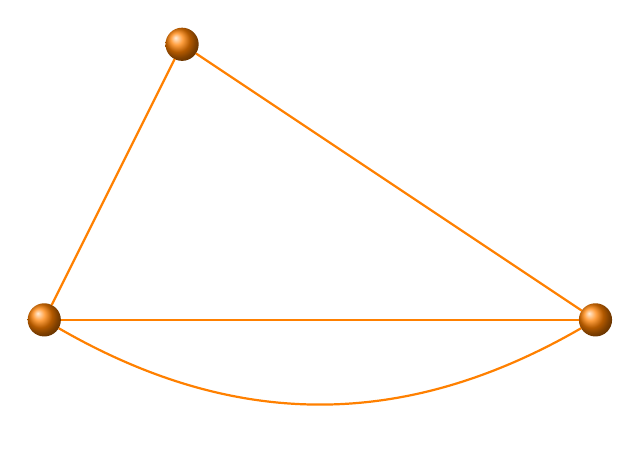
\begin{tikzpicture}[scale=1.75]
  \GraphInit[vstyle=Art]
  \Vertex{A}
  \Vertex[x=4,y=0]{B}
  \Vertex[x=1,y=2]{C}
  \Edge[style={bend left}](B)(A)
  \Edges(A,B,C,A)
\end{tikzpicture}
\end{document}
\end{tkzltxexample} 
\end{minipage}
\hfil\begin{minipage}{.40\textwidth}
  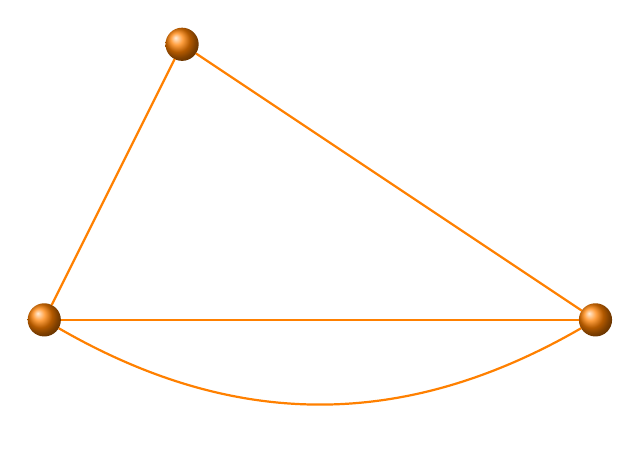
\begin{tikzpicture}[scale=1.75]
  \GraphInit[vstyle=Art]
  \Vertex{A}
  \Vertex[x=4,y=0]{B}
  \Vertex[x=1,y=2]{C}
  \Edge[style={bend left}](B)(A)
  \Edges(A,B,C,A)
\end{tikzpicture} 
  \end{minipage}
  
\newpage
\subsection{Exemple classique avec \tkzname{tkz-graph}}

Voyons un  exemple  classique. Nous allons utiliser un style  scolaire \tkzname{vstyle=Normal} ainsi que les macros \tkzcname{Vertices}, \tkzcname{NOEA} et \tkzcname{Edges} qui permet de créer une "chaîne" d'arêtes (edges). L'environnement \tkzname{scope} fait partie de \TIKZ, il est utilisé ici afin d'appliquer une rotation.

\begin{center}
\begin{tkzexample}[latex=7cm, small]
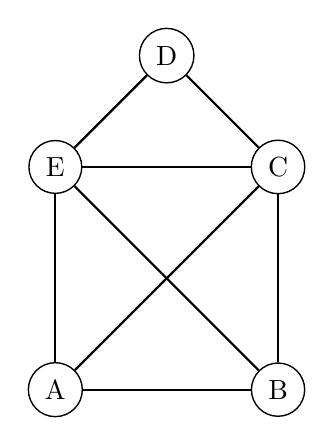
\begin{tikzpicture}
  \GraphInit[vstyle=Normal]
  \SetGraphUnit{2}
  \begin{scope}[rotate=-135]
      \Vertices{circle}{A,B,C,E}
  \end{scope}
  \NOEA[unit=1.414](E){D}
  \Edges(A,B,E,D,C,E,A,C,B)
\end{tikzpicture}
\end{tkzexample}
\end{center} 

\subsection{Modification du style}
Un style plus esthétique peut être choisi avec \tkzcname{GraphInit}. J'ai choisi \tkzname{Art} parmi une liste que vous découvrirez plus tard.

\begin{tkzexample}[latex=7cm,small]
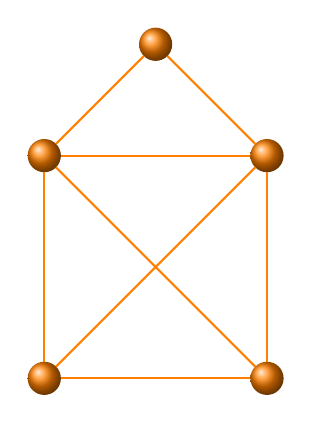
\begin{tikzpicture}
  \GraphInit[vstyle=Art]
  \begin{scope}[rotate=-135]
      \Vertices[unit=2]{circle}{A,B,C,E}
  \end{scope}
  \NOEA[unit=1.414](E){D}
  \Edges(A,B,E,D,C,E,A,C,B)
\end{tikzpicture}
\end{tkzexample}

\subsection{La ville de Königsberg avec \tkzname{tkz-graph}}


\begin{tkzexample}[latex=8cm]
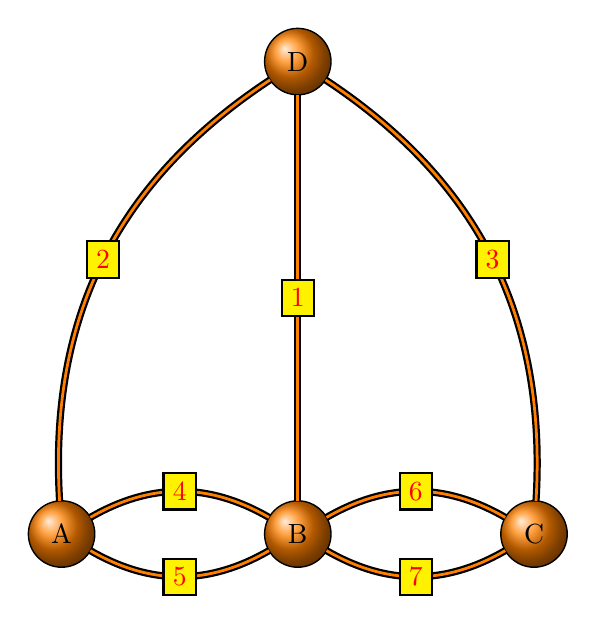
\begin{tikzpicture}
 \SetGraphUnit{3}
 \GraphInit[vstyle=Shade]
 \tikzset{LabelStyle/.style= {draw,
                              fill  = yellow,
                              text  = red}}
 \Vertex{A}
 \EA(A){B}
 \EA(B){C}
 \SetGraphUnit{6}
 % modifie la distance entre les nodes
 \NO(B){D}
 \Edge[label=1](B)(D)
 \tikzset{EdgeStyle/.append style = {bend left}}
 \Edge[label=4](A)(B)
 \Edge[label=5](B)(A)
 \Edge[label=6](B)(C)
 \Edge[label=7](C)(B)
 \Edge[label=2](A)(D)
 \Edge[label=3](D)(C)
\end{tikzpicture}
\end{tkzexample} 




\medskip
Ce dernier exemple était important sur un plan historique, mais il était un peu compliqué car on doit modifier des styles.

\subsection{La ville de Königsberg avec \TIKZ\ mais sans \tkzname{tkz-graph}}

Voyons l'exemple précédent, sans l'utilisation du package \tkzname{tkz-graph}.
L'exemple peut être vu sur cet excellent site \url{http://www.texample.net/tikz/examples/bridges-of-konigsberg/}, voici le code complet. The result is on the next page.
D'abord le préambule

\begin{tkzltxexample}[left margin=3cm,right margin=3cm]
% The seven bridges of Königsberg
% Author : Alain Matthes
% Encoding : UTF8
% Engine : PDFLaTeX
\documentclass[border=3mm]{standalone}
\usepackage{fullpage}
\usepackage{tikz}
\usetikzlibrary{arrows,shapes,positioning}                
\begin{document}
\end{tkzltxexample}

Ensuite les styles principaux

\begin{tkzltxexample}[left margin=3cm,right margin=3cm] 
\begin{center}
\begin{tikzpicture}
  \useasboundingbox (-1,-1) rectangle (11,11); 
  \tikzset{VertexStyle/.style = {shape          = circle,
                                 ball color     = orange,
                                 text           = black,
                                 inner sep      = 2pt,
                                 outer sep      = 0pt,
                                 minimum size   = 24 pt}}
  \tikzset{EdgeStyle/.style   = {thick,
                                 double          = orange,
                                 double distance = 1pt}}
  \tikzset{LabelStyle/.style =   {draw,
                                  fill           = yellow,
                                  text           = red}}
\end{tkzltxexample}
 
 enfin, le tracé
\begin{tkzltxexample}[left margin=3cm,right margin=3cm] 
     \node[VertexStyle](A){A};
     \node[VertexStyle,right=of A](B){B};
     \node[VertexStyle,right=of B](C){C};
     \node[VertexStyle,above= 7 cm of B](D){D};     
     \draw[EdgeStyle](B) to node[LabelStyle]{1} (D) ;
     \tikzset{EdgeStyle/.append style = {bend left}}
     \draw[EdgeStyle](A) to node[LabelStyle]{2} (B);
     \draw[EdgeStyle](B) to node[LabelStyle]{3} (A);
     \draw[EdgeStyle](B) to node[LabelStyle]{4} (C);
     \draw[EdgeStyle](C) to node[LabelStyle]{5} (B);
     \draw[EdgeStyle](A) to node[LabelStyle]{6} (D);
     \draw[EdgeStyle](D) to node[LabelStyle]{7} (C);
  \end{tikzpicture}
\end{center}
\end{document}
\end{tkzltxexample}

\begin{center}
\begin{tikzpicture}[scale=.75]
  \useasboundingbox (-1,-1) rectangle (11,11); 
  \tikzset{VertexStyle/.style = {shape          = circle,
                                 ball color     = orange,
                                 text           = black,
                                 inner sep      = 2pt,
                                 outer sep      = 0pt,
                                 minimum size   = 24 pt}}
  \tikzset{EdgeStyle/.style   = {thick,
                                 double          = orange,
                                 double distance = 1pt}}
  \tikzset{LabelStyle/.style =   {draw,
                                  fill           = yellow,
                                  text           = red}}   

     \node[VertexStyle](A){A};
     \node[VertexStyle,right= 4cm of A](B){B};
     \node[VertexStyle,right= 4cm of B](C){C};
     \node[VertexStyle,above= 7 cm of B](D){D};     
     \draw[EdgeStyle](B) to node[LabelStyle]{1} (D) ;
     \tikzset{EdgeStyle/.append style = {bend left}}
     \draw[EdgeStyle](A) to node[LabelStyle]{2} (B);
     \draw[EdgeStyle](B) to node[LabelStyle]{3} (A);
     \draw[EdgeStyle](B) to node[LabelStyle]{4} (C);
     \draw[EdgeStyle](C) to node[LabelStyle]{5} (B);
     \draw[EdgeStyle](A) to node[LabelStyle]{6} (D);
     \draw[EdgeStyle](D) to node[LabelStyle]{7} (C);
\end{tikzpicture}
\end{center}

\endinput